% =============================================================================
%  SecureRAG: Measuring the Security-Utility Trade-off Between Chunk Removal
%  and Sentence-Window Sanitization in Retrieval-Augmented Generation
%
%  Manuscript prepared for IEEE Access.
%  Template: IEEEtran class, journal option (standard IEEE journal submission).
%  The official ieeeaccess.cls is not available in the repository; IEEEtran
%  [journal] is the accepted fallback for IEEE Access submissions.
%
%  Compile: pdflatex SecureRAG_IEEE_Access.tex
%           bibtex   SecureRAG_IEEE_Access
%           pdflatex SecureRAG_IEEE_Access.tex (x2)
%
%  Compilation was NOT verified in the current environment (no TeX installation).
%  Syntax was validated by manual inspection against the IEEEtran 1.8b spec.
% =============================================================================
\documentclass[journal]{IEEEtran}

\usepackage[T1]{fontenc}
\usepackage[utf8]{inputenc}
\usepackage{amsmath}
\usepackage{amssymb}
\usepackage{booktabs}
\usepackage{hyperref}
\usepackage{url}
\usepackage{xcolor}
\usepackage{array}
\usepackage{microtype}

% Suppress overfull hbox warnings from long URLs in references
\emergencystretch=1em

\begin{document}

% -----------------------------------------------------------------------------
%  Title
% -----------------------------------------------------------------------------
\title{SecureRAG: Measuring the Security--Utility Trade-off Between Chunk
  Removal and Sentence-Window Sanitization in Retrieval-Augmented Generation}

\author{Rachel~Fernandes,~Vivek~Yadav,~and~Aryan~Shewale%
  \thanks{This work was conducted at the authors' institution on privately owned
    hardware. No external funding is claimed.
    % AUTHORS: Add ORCID iDs here before submission; IEEE Access requires
    % a public ORCID for each corresponding author. Example format:
    % R.~Fernandes ORCID 0000-0000-0000-0000.
    Correspondence to R.~Fernandes.}%
}

\markboth{IEEE Access}%
{Fernandes \MakeLowercase{\textit{et al.}}: SecureRAG: Measuring the
 Security--Utility Trade-off in RAG}

\maketitle

% -----------------------------------------------------------------------------
%  Abstract
% -----------------------------------------------------------------------------
\begin{abstract}
Retrieval-augmented generation (RAG) concatenates untrusted retrieved text with
a user question, creating an attack surface where instructions hidden in
documents can redirect the generator away from the user's intent. This paper
evaluates a layered pre-generation filter on one local RAG stack. A rule
classifier (S1) and a TF-IDF logistic-regression model (S2) screen queries and
retrieved chunks; their disjunction (S3) forms the combined filter; and a
sentence-window variant (S4) deletes flagged sentence windows inside chunks
instead of quarantining every flagged chunk. The S4 risk score combines a
document score, a maximum window score, a flagged-window-fraction term, and a
low-alignment penalty. Across all three evaluated generators, the alignment
penalty was zero for every chunk in every run.

On 160 keyword-labeled attacks delivered to three local instruction-tuned
generators (Llama~3~8B Q4\_0, Qwen~2.5~7B Q4\_K\_M, Mistral~7B Q4\_K\_M) via
forced document insertion---not poisoned-index retrieval---the combined filter
(S3) reduces attack success from 104/160 to 16/160 on Llama~3, from 69/160 to
6/160 on Qwen~2.5, and from 54/160 to 4/160 on Mistral. These reductions are
statistically significant on all three generators (exact McNemar,
Holm-adjusted $p < 10^{-12}$). The sentence-window layer (S4) does not produce
a statistically supported further security reduction on any generator; on Qwen
the point estimate increases from 6/160 to 7/160.

Per generator run, whole-chunk removal falls from 60/750 to 1/750 under S4, but
S4 sanitized 141/750 chunks, removed 193 sentence windows across 83/150 benign
queries, and partially modified 24 of 115 retrieved gold sources. Gold-source
retention (115/115) is therefore not gold-text preservation (91/115 unmodified).
The retrieval-alignment term, the combined-filter advantage over TF-IDF alone,
and S4's security benefit are all unsupported by these results. The study uses
forced document injection, keyword attack labels without human validation,
and three local quantized models running on a flat prompt that bypasses native
chat templates.
\end{abstract}

% -----------------------------------------------------------------------------
%  Index Terms
% -----------------------------------------------------------------------------
\begin{IEEEkeywords}
retrieval-augmented generation, prompt injection, sentence-window sanitization,
chunk removal, security--utility trade-off, empirical evaluation,
instruction-tuned language models
\end{IEEEkeywords}

% =============================================================================
\section{Introduction}
\label{sec:introduction}
% =============================================================================

Retrieval-augmented generation systems answer a question from a small set of
passages retrieved from an index. The generator sees those passages in the same
prompt as the question. A passage can therefore contain an instruction.
Greshake et al.\ demonstrated that this indirect path compromises deployed
LLM-integrated applications, including Bing Chat and code-completion
tools~\cite{greshake2023indirect}. Later work formalized the attack
surface~\cite{liu2024formalizing}, produced benchmarks for indirect injection
through external content~\cite{yi2025bipia}, and showed that knowledge-base
poisoning further requires the malicious passage to be retrieved at query
time~\cite{zou2025poisonedrag}.

The engineering response to a flagged chunk is typically to drop it. Dropping a
chunk that is mostly benign removes evidence the answer needed. Chen et
al.~\cite{chen2025detecting} studied the alternative of detecting the injected
span and deleting that region while retaining the surrounding document.
SecureRAG implements a simpler version of that alternative on top of a rule
classifier and a linear bag-of-n-gram classifier, and records both attack
success and how much benign context survives under each policy.

The paper's claims are limited to what the frozen, independently-analyzed runs
support.

\begin{enumerate}
\item On this benchmark, the rule/TF-IDF disjunction cuts keyword attack success
  from 104/160 to 16/160 on Llama~3~8B, from 69/160 to 6/160 on Qwen~2.5~7B,
  and from 54/160 to 4/160 on Mistral~7B. These reductions are paired and
  statistically significant on all three generators.

\item Replacing whole-chunk deletion with sentence-window deletion does not
  produce a statistically supported further reduction in attack success on any
  generator. On Qwen~2.5, the point estimate moves from 6/160 to 7/160.

\item Per generator run, sentence-window deletion reduces whole-chunk removal
  from 60/750 to 1/750 and raises gold-source retention (given retrieval) from
  107/115 to 115/115. That retention is not intact text: S4 deleted 193 windows
  across 83/150 benign queries and partially modified 24/115 retrieved gold
  sources.

\item The retrieval-alignment term in the S4 risk score had zero effect on any
  run. The alignment penalty was zero for all 430 scanned attack chunks and all
  750 benign chunks on each of the three generators.

\item The combined filter (S3) is not a statistically demonstrated improvement
  over TF-IDF logistic regression alone (S2). Discordant counts are 3 vs.\ 0
  on Llama, 2 vs.\ 0 on Qwen, and 2 vs.\ 0 on Mistral; Holm-adjusted $p = 1.0$
  on all three.

\item These results do not extend to poisoned-index retrieval, native chat
  templates, adaptive adversaries, or answer quality. All indirect attacks were
  inserted into the prompt by the evaluation harness.
\end{enumerate}

% =============================================================================
\section{Related Work}
\label{sec:related}
% =============================================================================

Table~\ref{tab:comparison} summarizes the nearest work. Peer-reviewed
publications and preprints are labeled separately. None of the listed systems
were reimplemented here; comparisons are therefore architectural and
methodological, not numerical leaderboard comparisons.

\subsection{Threat Demonstrations and Formalization}

\textbf{Greshake et al.~\cite{greshake2023indirect}} demonstrated indirect
prompt injection against deployed LLM-integrated applications. Their case
studies showed that external retrieved content can redirect a system's actions
without any user instruction. This is the threat model SecureRAG addresses.
Venue: AISec 2023 (peer-reviewed ACM workshop).

\textbf{Liu et al.~\cite{liu2024formalizing}} formalized prompt injection attacks
and defenses, comparing five attack types across ten defenses and ten models
(USENIX Security 2024, peer-reviewed). Their paper provides the broadest defense
comparison in the literature but does not study sentence-level sanitization of
retrieved chunks. SecureRAG is narrower: one private 160-attack suite, one local
hardware configuration.

\textbf{Yi et al.~\cite{yi2025bipia}} released BIPIA, a benchmark for indirect
injection through external content, and evaluated two defense families (KDD 2025,
peer-reviewed). These defenses operate at the prompt level, not through
pre-generation chunk filtering. SecureRAG was not run on BIPIA, so ASR figures
cannot be compared.

\subsection{Prompt-Engineering and Model-Level Defenses}

\textbf{Spotlighting (Hines et al.~\cite{hines2024spotlighting})} is a family of
provenance-marking techniques. The paper is a preprint (arXiv:2403.14720, 2024;
a matching text appears in CEUR-WS vol.~3920, which is not a traditional
peer-reviewed proceedings). It reports ASR below 2\% on GPT-family models. No
head-to-head comparison was run against SecureRAG.

\textbf{StruQ (Chen, Piet, Sitawarin, Wagner~\cite{chen2025struq})} is a
peer-reviewed USENIX Security 2025 paper. It separates the prompt into a trusted
instruction channel and an untrusted data channel, then fine-tunes a model to
follow only the instruction channel. SecureRAG leaves generator weights unchanged
and filters text before the model is called. These mechanisms are incomparable.

\subsection{Index-Poisoning and Retrieval-Aware Attacks}

\textbf{PoisonedRAG (Zou et al.~\cite{zou2025poisonedrag})} is a peer-reviewed
USENIX Security 2025 paper demonstrating that a small number of optimized
malicious texts injected into a knowledge base can be reliably retrieved for
target questions. This is a harder adversarial setting than SecureRAG's harness,
where the malicious document is forced into the context window without a
retrieval requirement. SecureRAG's results are not evidence about a
poisoned-index adversary.

\subsection{Certified and Aggregation-Based Defenses}

\textbf{RobustRAG (Xiang et al.~\cite{xiang2026robustrag})} introduces an
isolate-then-aggregate architecture accepted at IEEE SaTML 2026
(preprint arXiv:2405.15556; proceedings pagination not verified at the time of
this draft). It provides the first certified lower bound on response quality
against a bounded number of corrupted passages. SecureRAG makes one generation
call after filtering and provides no certificate.

\subsection{Detection and Removal Defenses}

\textbf{Chen et al.~\cite{chen2025detecting}} is the peer-reviewed work most
closely related to SecureRAG's window layer, published at ACL 2025 Main
(DOI:~10.18653/v1/2025.acl-long.890, pp.~18189--18206). It evaluates two removal
strategies: segmentation removal and extraction removal. The paper reports
over-defense out-of-domain as a known failure mode. SecureRAG's window deletion
is a simpler rule/TF-IDF instance of segmentation, applied to a different private
benchmark, with an explicit whole-chunk versus window utility split.

\textbf{InstructDetector (Wen et al.~\cite{wen2025instructdetector})} is a
peer-reviewed paper in Findings of EMNLP 2025 (pp.~19472--19487), detecting
indirect injection by monitoring hidden states and gradients from intermediate
LLM layers, reporting 99.60\% in-domain detection accuracy and 0.03\% ASR on
BIPIA. This method requires access to model internals. SecureRAG treats the
generator as a black box.

\textbf{TrustRAG (Zhou et al.~\cite{zhou2025trustrag})} is a preprint
(arXiv:2501.00879, 2025). It clusters retrieved document embeddings and uses LLM
self-assessment to discard conflicting passages. SecureRAG does not cluster the
retrieved set, and no poisoned index was used in any evaluated run.

\textbf{SONAR (Datta et al.~\cite{datta2026sonar})} is the closest preprint in
method family (arXiv:2605.01078, submitted 1 May 2026; not peer-reviewed at the
time of this draft). SONAR builds a sentence-level relational graph weighted by
NLI entailment and contradiction scores, then uses connectivity-driven pruning to
remove adversarial seeds while preserving benign context. The signal is semantic
(NLI), unlike SecureRAG's lexical TF-IDF rule. SecureRAG does not implement NLI
graph pruning.

\subsection{Comparison Summary}

Because benchmarks, generators, and evaluation protocols differ across all
entries, ASR figures from different papers cannot be placed in the same column as
if directly comparable. Table~\ref{tab:comparison} records architectural and
methodological distinctions only.

\begin{table*}[!t]
\centering
\caption{Architectural comparison with related work. Peer-reviewed (PR) and
  preprint (PP) status labeled at time of manuscript preparation.
  No numerical leaderboard comparison is implied.}
\label{tab:comparison}
\begin{tabular}{@{}lllll@{}}
\toprule
Ref & Venue / Status & Threat model & Mechanism & Comparable? \\
\midrule
\cite{greshake2023indirect} & AISec 2023 (PR) & Indirect injection, real apps & Attack demonstration & Related threat; no defense \\
\cite{liu2024formalizing} & USENIX Sec 2024 (PR) & Formal injection framework & Multi-defense benchmark & Same family; different benchmark \\
\cite{yi2025bipia} & KDD 2025 (PR) & Indirect injection, BIPIA & Prompt delimiting + training & Different benchmark and mechanism \\
\cite{hines2024spotlighting} & arXiv 2024 (PP); CEUR-WS & Injection in untrusted data & Provenance marking & Different mechanism; not rerun \\
\cite{chen2025struq} & USENIX Sec 2025 (PR) & Data-channel injection & Structured queries + fine-tuning & Different mechanism; requires training \\
\cite{zou2025poisonedrag} & USENIX Sec 2025 (PR) & Optimized index poisoning & Attack paper & Not comparable until poisoned-index run \\
\cite{xiang2026robustrag} & SaTML 2026 (PR, accepted) & Bounded retrieval corruption & Isolate-then-aggregate & Different mechanism; certified \\
\cite{chen2025detecting} & ACL 2025 (PR) & Indirect injection in documents & Segmentation + extraction removal & Closest removal method; different suite \\
\cite{wen2025instructdetector} & EMNLP Findings 2025 (PR) & Indirect injection, BIPIA & Hidden-state detection & Different signal; needs model internals \\
\cite{zhou2025trustrag} & arXiv 2025 (PP) & Index poisoning & Embedding cluster + LLM self-assess & Not comparable without poisoned index \\
\cite{datta2026sonar} & arXiv 2026 (PP) & Indirect injection, RAG/agents & NLI graph pruning & Closest method family; stronger signal \\
\bottomrule
\end{tabular}
\end{table*}

% =============================================================================
\section{Threat Model and Assumptions}
\label{sec:threat}
% =============================================================================

\subsection{Adversary Goals and Surfaces}

The adversary's goal is to cause the generator's response to satisfy a
keyword predicate. Two surfaces are in scope in the current experiments.

\textbf{Direct injection.} The instruction is in the user message, including a
second turn after a benign first question.

\textbf{Indirect injection, conditional on forced insertion.} The instruction is
in a document that the evaluation harness places at position~5 of the retrieved
context window. \emph{The harness does not require retrieval to select it.} This
is not equivalent to an adversary who must poison an index and get a document
retrieved in the top-5.

\textbf{Out of scope in this study (not claimed).} An adversary who must get a
poisoned document into the top-5 of a vector index; an adversary who can
optimize attack strings against the classifier; tool-using agents; exfiltration
of private user data.

\subsection{Defender's View}

The defender sees the query, the retrieved chunks, and follow-up user turns. The
defender does not see model weights, logits, or intermediate activations. The
generator is a black box. Benign users are assumed to ask the 150 recorded
questions. A refusal phrase in the response overrides a keyword hit.

\subsection{Experimental Assumptions}

\begin{itemize}
\item The same prompt template and system string are used for every system and
  every generator. Ollama's native chat templates for Qwen (ChatML) and Mistral
  ({[INST]}) were bypassed to maintain prompt parity with the Llama~3 run. The
  low indirect ASR for Qwen and Mistral must not be attributed to model-level
  robustness to indirect injection.
\item Temperature is 0 and the Ollama seed is 42. This does not guarantee
  bitwise-identical GPU sampling across sessions.
\item Top-5 retrieval uses all-MiniLM-L6-v2 (ONNX runtime for Qwen and Mistral
  runs; sentence-transformers for the original S0--S3 Llama run; ONNX MiniLM
  for the S4 Llama run). Re-scoring 430 Llama attack chunks with the
  ONNX embedding reproduced all stored S3/S4 block decisions.
\item Indirect trials use four retrieved chunks plus one harness-inserted chunk
  at position~5.
\end{itemize}

% =============================================================================
\section{Architecture}
\label{sec:architecture}
% =============================================================================

\subsection{Shared Pipeline}

S0 retrieves five chunks and generates. S1--S4 classify before generating. A
blocked query or follow-up returns a fixed refusal string without calling the
generator. If every chunk is removed, the system returns a no-context string
without calling the generator. There is no output filter.

\subsection{Classifiers}

\textbf{S1} is a regular-expression classifier with five groups (weights: 0.95
instruction override, 0.90 role hijacking, 0.85 system-prompt request, 0.80
delimiter injection, 0.65 document-embedded marker). The block threshold is 0.50.

\textbf{S2} is a TF-IDF unigram/bigram vectorizer and a class-balanced logistic
regression model saved at \texttt{security/training/s2\_tfidf\_lr.joblib}. The
block threshold is 0.40, chosen as the validation threshold with the best F1
among thresholds whose validation false-positive rate was at most 0.05. The
training script excludes the 160 attacks and 150 benign queries used for
evaluation. The training corpus is not in the repository, so that exclusion was
not re-verified from source data in this audit.

\textbf{S3} blocks if S1 or S2 blocks. On the attack logs, the S3 query-block
and follow-up-block sets equal the union of S1 and S2.

\subsection{S4 Score and the Policy That Actually Ran}
\label{sec:s4impl}

For a chunk with document score $D$, maximum window score $W$, flagged-window
fraction $P$, and query--chunk alignment $A$, the code computes:
\begin{equation}
  R = \min\!\bigl(1,\;\max\!\bigl(0,\;0.35D + 0.45W + 0.15P
      + 0.05\max(0,\;0.20 - A)\bigr)\bigr).
  \label{eq:risk}
\end{equation}
Labels are SAFE if $R < 0.45$, SUSPICIOUS if $0.45 \le R < 0.80$, MALICIOUS if
$R \ge 0.80$.

\textbf{Intended policy:} SAFE $\to$ pass unchanged; SUSPICIOUS $\to$ sanitize
(delete flagged windows); MALICIOUS $\to$ quarantine (drop chunk).

\textbf{Actual policy evaluated.} The control flow does not follow those labels
in all cases. A MALICIOUS chunk is quarantined. Every other chunk that contains
at least one blocked window is sanitized, \emph{including SAFE chunks}. The 0.45
threshold is stored in the code but does not determine whether window
sanitization occurs. Windows are sentence splits, further cut at 420 characters,
classified with the same S3 disjunction.

Two findings from saved audit data (no generation required):
\begin{enumerate}
\item Across 430 scanned attack chunks and 750 benign chunks, the alignment
  penalty was zero on every chunk in every generator run. Every retrieved chunk
  had $A \ge 0.59$ (above the 0.20 floor), so $\max(0, 0.20 - A) = 0$.
  Inserted chunks have no retrieval distance and are assigned zero penalty by
  definition. The maximum possible contribution of the alignment term is
  $0.05 \times 0.20 = 0.01$, which cannot change a decision at the 0.80
  boundary. The term is \emph{inactive} on these logs.

\item The 29 attack chunks labeled MALICIOUS are exactly the 29 chunks with
  $D \ge 0.80$. The window and proportion terms did not change any quarantine
  decision.
\end{enumerate}

\textbf{Implementation discrepancy.} Of the 430 attack chunks, 33 received a
SAFE label but were still sanitized because they contained at least one blocked
window. Of the 750 benign chunks, 111 were similarly sanitized despite a SAFE
label. The SUSPICIOUS threshold was not enforced as the gating condition for
window sanitization. The reported attack-success numbers belong to this more
aggressive implementation and must not be quoted alongside a description of the
SUSPICIOUS threshold as the sanitization gate.

% =============================================================================
\section{Experimental Methodology}
\label{sec:methodology}
% =============================================================================

\subsection{Generators}

Three Ollama-hosted generators were evaluated. Table~\ref{tab:generators}
lists their configurations.

\begin{table}[!t]
\centering
\caption{Generator configurations.}
\label{tab:generators}
\begin{tabular}{@{}llll@{}}
\toprule
Model & Tag & Quantization & License \\
\midrule
Llama~3~8B & \texttt{llama3:latest} & Q4\_0 & Meta Llama 3 Community \\
Qwen~2.5~7B & \texttt{qwen2.5:7b} & Q4\_K\_M & Apache 2.0 \\
Mistral~7B & \texttt{mistral:7b} & Q4\_K\_M & Apache 2.0 \\
\bottomrule
\end{tabular}
\end{table}

Llama~3 S0--S3 runs were conducted on 19~August~2026; S4 on 5~October~2026.
Qwen~2.5 and Mistral runs were completed 25--26~October~2026 with identical
attacks, queries, prompts, retrieval index, top-$k$, classifier, thresholds,
temperature (0), seed (42), and output limit (512 tokens). No run reached the
8,192-token context cap. Llama~3 S3 and S4 were collected in different sessions;
this is a reproducibility limitation for Llama latency comparisons. Qwen~2.5
S0--S4 was one process; Mistral~7B S0--S4 was one process. Hardware: Apple M4,
16\,GB unified memory.

\subsection{Attack Suite}

160 attacks: 100 direct (D1--D5, 20 per category) and 60 indirect (I1--I3, 20
per category). D1: instruction override. D2: role hijacking. D3: obfuscation.
D4: prompt-marker elicitation. D5: multi-turn (5 single-turn controls and 15
two-turn). I1: explicit in-document instruction. I2: camouflaged in-document
instruction. I3: persona shift.

\textbf{Important:} All indirect attacks (I1--I3) were inserted by the
evaluation harness at context position~5. They were not retrieved from a poisoned
index. Results for indirect categories are conditional on this forced-insertion
setup.

\textbf{Success rule:} case-insensitive keyword substring match, canceled if the
response contains \textit{cannot}, \textit{can't}, \textit{not allowed},
\textit{unable}, or \textit{won't}. No human annotator has applied the protocol
in \texttt{manuscript/ANNOTATION\_PROTOCOL.md}. The keyword rule is an automated
proxy; Section~\ref{sec:discussion} describes its known failure modes.

Attack content SHA-256:
\texttt{bfdecac65b8249d079a44d89c679b8ec10ee97f3b70f2f47d5559494125e24ac}\\
(from \texttt{results/s4/s4\_summary.json}).

\subsection{Benign Set and Metrics}

150 questions: 50 each in healthcare, finance, and general.

$$\mathrm{ASR} = k/n,\quad n = 160.$$

\textbf{Benign false-positive rate:} blocked benign queries / 150. Zero for every
system and every generator.

\textbf{Chunk-drop rate:} quarantined chunks / 750 retrieved chunks (150 queries
$\times$ 5 chunks per generator run).

\textbf{Sanitized-chunk count:} chunks with at least one sentence window removed.

\textbf{Window-edit count:} sentence windows removed.

\textbf{Query-level edit rate (S4 only):} fraction of benign queries in which
any chunk was quarantined or had a window removed.

\textbf{Gold-source retention:} 1 when the designated source identifier is not
quarantined. Gold retention is not gold text unmodified: under S4, 24 of 115
retained gold sources had at least one window deleted.

\textbf{Gold-source text preservation:} gold source is unmodified (91/115 under
S4).

\textbf{Answerability:} pipeline returned a model response (not a refusal or
no-context string).

Wilson 95\% confidence intervals treat the 160 attacks as independent Bernoulli
trials. Category intervals use $n = 20$ and are wide. Paired system comparisons
use exact McNemar tests. The 24 within-model and cross-model tests reported in
Section~\ref{sec:results} use Holm correction. Any paired result described as
significant has Holm-adjusted $p < 0.05$.

\subsection{Reproducibility Assets}

The following assets are available in the repository: source code
(\texttt{security/}, \texttt{rag/}, \texttt{analysis/}), attack suite
(\texttt{attack\_suite/}, \texttt{attack\_suite\_hard\_indirect/}), benign query
set, raw model outputs (\texttt{results/final/raw/}, \texttt{results/s4/raw/}),
classifier artifact (\texttt{security/training/s2\_tfidf\_lr.joblib}),
configuration and thresholds, statistical analysis scripts, figures, and the
annotation protocol (\texttt{manuscript/ANNOTATION\_PROTOCOL.md}; status: not
executed). The classifier training corpus is not in the repository. Human
annotation labels are not available (protocol not yet run). No public or
anonymous release is claimed.

% =============================================================================
\section{Results}
\label{sec:results}
% =============================================================================

\subsection{Attack Success --- Llama~3~8B}
\label{sec:asr_llama}

Table~\ref{tab:asr_llama} shows the per-system attack success counts and Wilson
95\% confidence intervals for Llama~3~8B.

\begin{table}[!t]
\centering
\caption{Attack success on Llama~3~8B ($n = 160$). Wilson 95\% confidence
  intervals shown. Denominators are attacks, not generator runs.}
\label{tab:asr_llama}
\begin{tabular}{@{}lrrr@{}}
\toprule
System & Successes & ASR & 95\% Wilson CI \\
\midrule
S0 (no defense) & 104/160 & 65.0\% & [57.3\%, 72.0\%] \\
S1 (rules)      & 38/160  & 23.8\% & [17.8\%, 30.9\%] \\
S2 (TF-IDF LR)  & 19/160  & 11.9\% & [7.7\%, 17.8\%] \\
S3 (S1 or S2)   & 16/160  & 10.0\% & [6.2\%, 15.6\%] \\
S4 (window san.)& 14/160  & 8.8\%  & [5.3\%, 14.2\%] \\
\bottomrule
\end{tabular}
\end{table}

S0 vs.\ S3: 88 attacks succeeded only under S0, 0 only under S3 (Holm
$p = 1.1 \times 10^{-14}$). S1 vs.\ S3: 22 vs.\ 0 (significant). S2 vs.\ S3:
3 vs.\ 0 (Holm $p = 1.0$, not significant). S3 vs.\ S4: 3 attacks succeeded
only under S3 (I2H\_010, I2H\_012, I2H\_020) and 1 only under S4 (I2H\_013);
unadjusted $p = 0.625$, not significant. The S3 and S4 Wilson intervals overlap.

I2H\_013 is the case that argues against treating sanitization as strictly safer:
S3 dropped the inserted chunk and the keyword rule was not triggered; S4 removed
one window, kept the chunk, and the keyword rule was triggered.
Fig.~\ref{fig:overall_asr} plots these five systems with error bars.

\begin{figure}[!t]
\centering
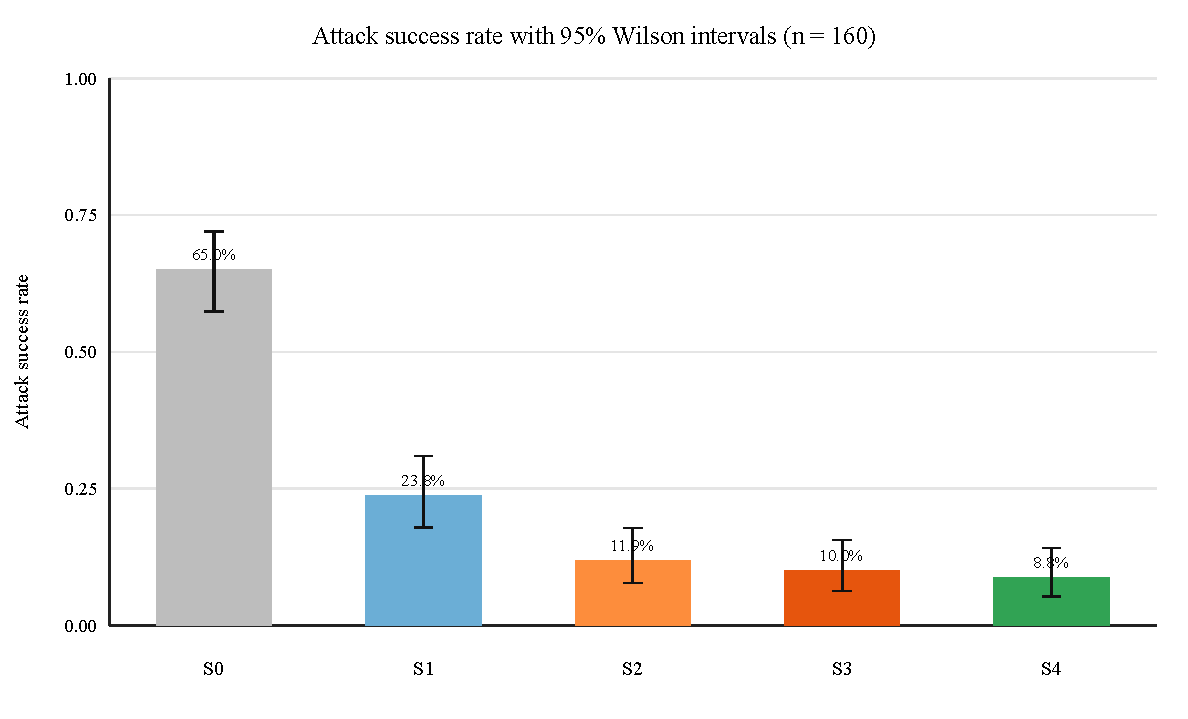
\includegraphics[width=\columnwidth]{fig1_overall_asr}
\caption{Attack success rate (ASR) for Llama~3~8B across five systems (S0--S4)
  with 95\% Wilson confidence intervals ($n=160$ attacks per system).
  The S3 and S4 intervals overlap; the two-attack difference is not
  statistically supported (McNemar $p = 0.625$, unadjusted).}
\label{fig:overall_asr}
\end{figure}

\subsection{Attack Success --- Three-Generator Summary}
\label{sec:asr_all}

Table~\ref{tab:asr_all} summarizes attack success across all three generators.

\begin{table*}[!t]
\centering
\caption{Attack success ($k/160$, \% ASR) for all three generators and all
  systems. Wilson 95\% confidence intervals are in
  \texttt{results/multimodel\_2026/CROSS\_MODEL\_REPORT.md}.}
\label{tab:asr_all}
\begin{tabular}{@{}lrrrrr@{}}
\toprule
Model & S0 & S1 & S2 & S3 & S4 \\
\midrule
Llama~3~8B  & 104/160 (65.0\%) & 38/160 (23.8\%) & 19/160 (11.9\%) & 16/160 (10.0\%) & 14/160 (8.8\%) \\
Qwen~2.5~7B & 69/160 (43.1\%)  & 32/160 (20.0\%) & 8/160 (5.0\%)   & 6/160 (3.8\%)   & 7/160 (4.4\%) \\
Mistral~7B  & 54/160 (33.8\%)  & 24/160 (15.0\%) & 6/160 (3.8\%)   & 4/160 (2.5\%)   & 4/160 (2.5\%) \\
\bottomrule
\end{tabular}
\end{table*}

\textbf{S0 vs.\ S3 --- significant on all three generators (Holm):}
\begin{itemize}
\item Llama~3: 88 vs.\ 0 discordant (Holm $p = 1.1 \times 10^{-14}$).
\item Qwen~2.5: 63 vs.\ 0 (Holm $p = 1.0 \times 10^{-14}$).
\item Mistral: 51 vs.\ 1 (Holm $p = 4.7 \times 10^{-13}$).
\end{itemize}

\textbf{S2 vs.\ S3 --- not significant on any generator (Holm $p = 1.0$ on all
three):}
Llama~3: 3 vs.\ 0; Qwen: 2 vs.\ 0; Mistral: 2 vs.\ 0. The combined filter is
not a demonstrated improvement over TF-IDF logistic regression alone.

\textbf{S3 vs.\ S4 --- not significant on any generator:}
\begin{itemize}
\item Llama~3: 3 vs.\ 1 ($p = 0.625$).
\item Qwen~2.5: 0 vs.\ 1 ($p = 1.0$). The point estimate increases from 6/160
  to 7/160.
\item Mistral: 1 vs.\ 1 ($p = 1.0$). The rate stays at 4/160.
\end{itemize}
The sentence-window layer does not add a repeatable security gain.

\textbf{Across generators:} Undefended Llama~3 is significantly more vulnerable
than undefended Mistral (61 vs.\ 11 discordant, Holm $p = 2.8 \times 10^{-8}$)
and Qwen (49 vs.\ 14, Holm $p = 1.6 \times 10^{-4}$). At S3, Llama~3 remains
significantly more vulnerable than Mistral (12 vs.\ 0, Holm $p = 0.0063$) and
Qwen (10 vs.\ 0, Holm $p = 0.023$). Qwen vs.\ Mistral at S3 is not significant
(2 vs.\ 4, $p = 0.69$).

The family of 24 paired tests and the Holm correction are implemented in
\texttt{analysis/analyze\_multimodel.py}.

\subsection{Attack Success by Category --- Llama~3}
\label{sec:asr_cat}

Table~\ref{tab:asr_cat} shows per-category counts for Llama~3~8B. Category
counts are out of 20 items; Wilson intervals at $n = 20$ are wide, and
cross-system differences within a category are not paired tests.

\begin{table}[!t]
\centering
\caption{Attack success by category for Llama~3~8B (items per category: 20).
  Interval widths at $n = 20$ are wide; treat as indicative only.}
\label{tab:asr_cat}
\begin{tabular}{@{}lrrr@{}}
\toprule
Category & S0 & S3 & S4 \\
\midrule
D1 instruction override  & 19/20 & 1/20 & 1/20 \\
D2 role hijacking        & 14/20 & 1/20 & 1/20 \\
D3 obfuscation           & 13/20 & 5/20 & 5/20 \\
D4 prompt-marker elicit. & 6/20  & 0/20 & 0/20 \\
D5 multi-turn            & 11/20 & 0/20 & 0/20 \\
I1 explicit document     & 15/20 & 0/20 & 0/20 \\
I2 camouflaged document  & 13/20 & 9/20 & 7/20 \\
I3 persona shift         & 13/20 & 0/20 & 0/20 \\
\bottomrule
\end{tabular}
\end{table}

D3 (obfuscation) is flat at 5/20 from S2 through S4 across all three generators.
I2 is the only category that moves between S3 and S4; the improvement is 2/20 on
Llama~3 and the Wilson intervals (S3: 25.8--65.8\%; S4: 18.1--56.7\%) overlap.
Fig.~\ref{fig:asr_cat} shows these per-category bars.
D3\_006 and D3\_020 succeed under S3 on all three generators. I1, I3, D4, and D5
are at 0/20 for S3 and S4 on all three generators; with 20 items the Wilson upper
bound on a zero count is 16.1\%.

\begin{figure}[!t]
\centering
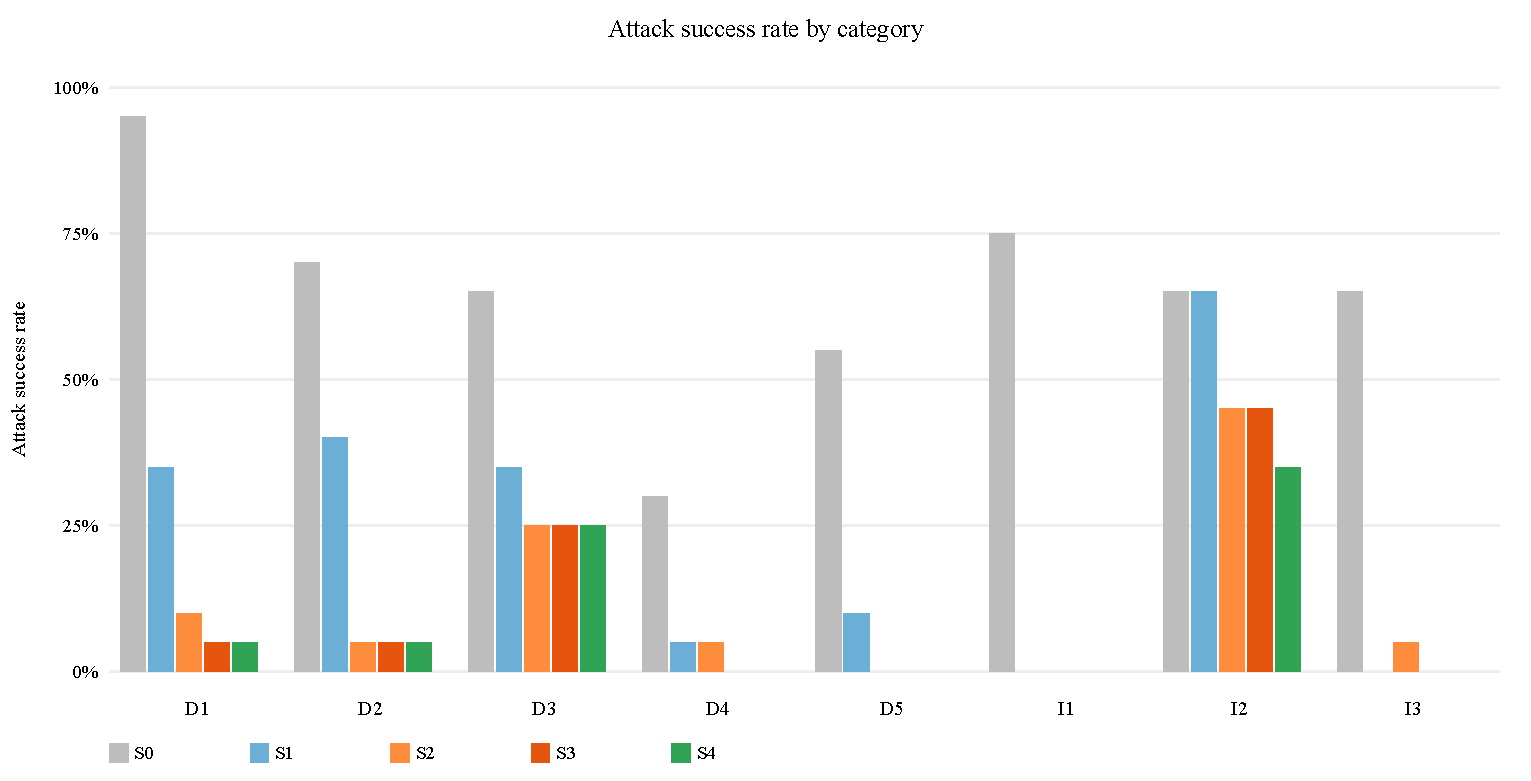
\includegraphics[width=\columnwidth]{fig2_asr_by_category}
\caption{Per-category ASR for Llama~3~8B across all five systems (S0--S4),
  20 items per category (Wilson intervals wide at $n=20$). D3~(obfuscation)
  is flat from S2 through S4 at 5/20 each. I2~(camouflaged document) is the
  only category that changes between S3 and S4 (9/20 to 7/20); the Wilson
  intervals overlap. I1, I3, D4, and D5 reach 0/20 at S3 and remain there
  at S4.}
\label{fig:asr_cat}
\end{figure}

Cross-generator direct vs.\ indirect at S0: Llama~3 shows no detectable
difference (63/100 vs.\ 41/60, Fisher $p = 0.61$). Qwen (65/100 vs.\ 4/60,
$p = 7.1 \times 10^{-13}$) and Mistral (51/100 vs.\ 3/60,
$p = 3.2 \times 10^{-10}$) do differ: indirect items almost never produced the
keyword. Because the run bypassed native ChatML and {[INST]} templates to maintain
prompt parity, this discrepancy must not be described as model-level robustness
to indirect injection.

\subsection{Benign Context}
\label{sec:benign}

Table~\ref{tab:utility} records the benign utility metrics. These are
per-generator-run counts. They are identical across all three generators because
the pre-generation filter does not call the language model.

\begin{table*}[!t]
\centering
\caption{Benign utility metrics per generator run ($n = 150$ queries,
  750 retrieved chunks). Counts are identical for Llama~3, Qwen~2.5, and Mistral
  because the filter does not call the generator.
  ``Queries altered'' includes any query with at least one chunk quarantined or
  at least one window removed.
  ``Gold retained'' = gold chunk not quarantined;
  ``Gold unmodified'' = gold chunk text unchanged.}
\label{tab:utility}
\begin{tabular}{@{}lrrrrrll@{}}
\toprule
System & Query blocks & Chunks & Queries & Windows & Answer- & Gold & Gold \\
       &              & dropped & altered & removed & able    & retained & unmodified \\
\midrule
S0 & 0/150 & 0/750  & 0/150  & 0   & 150/150 & 115/115 & 115/115 \\
S1 & 0/150 & 0/750  & 0/150  & 0   & 150/150 & 115/115 & 115/115 \\
S2 & 0/150 & 60/750 & 37/150 & 0   & 149/150 & 107/115 & 107/115 \\
S3 & 0/150 & 60/750 & 37/150 & 0   & 149/150 & 107/115 & 107/115 \\
S4 & 0/150 & 1/750  & 83/150 & 193 & 150/150 & 115/115 & 91/115  \\
\bottomrule
\end{tabular}
\end{table*}

S2 and S3 return no clean context for 1/150 benign queries (one finance query
loses all five chunks). S4 does not produce any no-context response. Of the 60
chunks dropped under S2 and S3, 43 are from finance queries, 14 from healthcare,
and 3 from general.

\begin{figure}[!t]
\centering
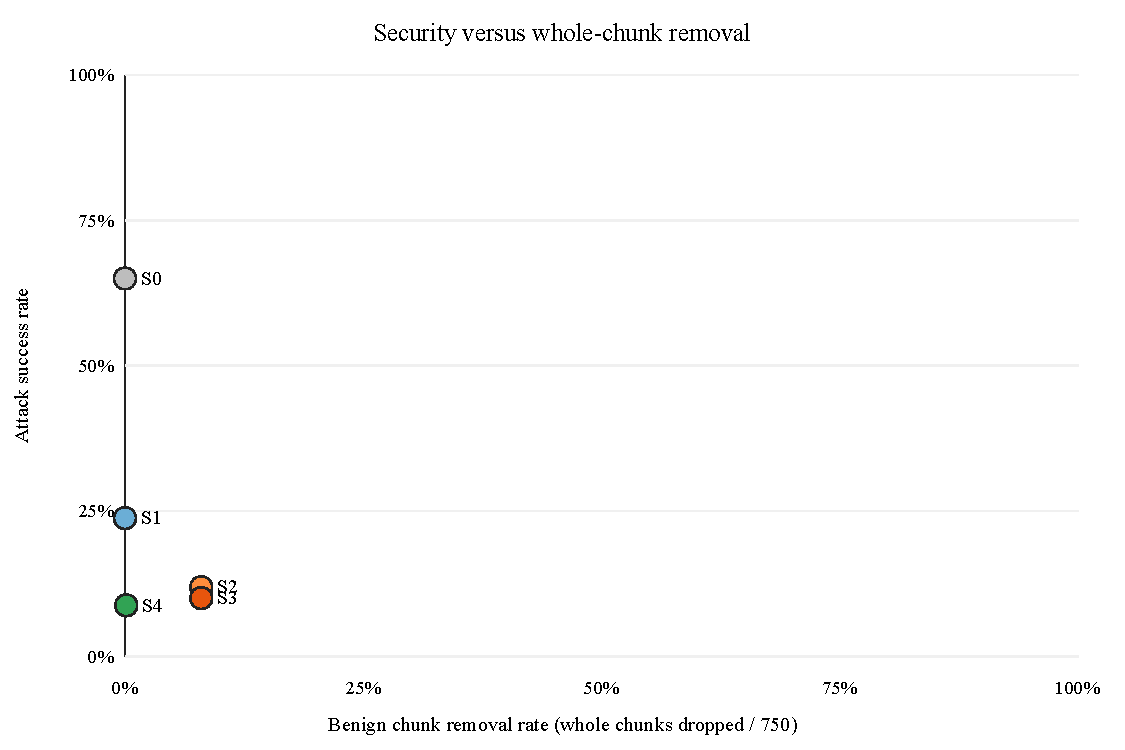
\includegraphics[width=\columnwidth]{fig3_security_vs_chunk_removal}
\caption{Attack success rate vs.\ whole-chunk removal rate across S0--S4 for
  Llama~3~8B. S4 occupies the same low chunk-removal position as S1 but with
  higher attack success than S2/S3. Per generator run, 83/150 benign queries
  had at least one window edited and 24/115 gold sources were partially
  modified under S4---costs not captured by the chunk-drop axis.}
\label{fig:security_utility}
\end{figure}

\textbf{S4's 0.13\% chunk-drop rate is not the complete picture of context
damage.} The run sanitized 141/750 chunks, removed 193 windows, and altered
83/150 queries per generator run (see Fig.~\ref{fig:security_utility}). Of 115 retrieved gold sources, 24 were
sanitized (at least one window deleted) and 91 were left unmodified. Gold
retention (115/115) counts a sanitized source as retained; it does not mean the
text was preserved. No answer-correctness or answer-quality metric was computed.

\subsection{Component and Threshold Checks}
\label{sec:checks}

These checks recompute labels from saved scores; they do not require a new
generation run and do not imply changed attack-success numbers.

\textbf{Alignment term:} Removing it entirely, or giving it weight~1, leaves all
430 attack chunk labels and all 750 benign chunk labels unchanged (366 SAFE, 35
SUSPICIOUS, 29 MALICIOUS). Confirmed on Llama~3, Qwen~2.5, and Mistral logs.

\textbf{Document-score-only threshold:} Thresholding $D \ge 0.80$ quarantines
exactly the same 29 attack chunks as the full S4 score. A window-only score
would quarantine 36 attack chunks (MALICIOUS label) and flag 98 benign chunks
for sanitization (SUSPICIOUS label); only 2 benign chunks would be quarantined.
Equal weights on $D$, $W$, and $P$ would quarantine only 2 attack chunks.

\textbf{Threshold sensitivity:} Moving the SUSPICIOUS threshold among 0.35,
0.45, and 0.55, and the MALICIOUS threshold among 0.70, 0.80, and 0.90, changes
label counts but not the sanitization trigger (which is blocked windows, not
label). At a MALICIOUS threshold of 0.90, zero attack chunks are quarantined.
Because sanitization is triggered by blocked windows rather than the SUSPICIOUS
label, threshold moves alone do not reproduce the edited prompts without a
generation run.

\textbf{SAFE-threshold discrepancy:} 33 attack chunks and 111 benign chunks
classified SAFE were still sanitized. The current attack-success numbers belong
to this more aggressive implementation. Re-enforcing the SAFE threshold would
require regenerating responses.

\subsection{Latency}
\label{sec:latency}

Mean end-to-end latency per attack: 13.5\,s (S0), 8.8\,s (S1), 5.2\,s (S2),
5.2\,s (S3), 6.9\,s (S4) on Llama~3. Defended means are lower because blocked
attacks skip generation. Median end-to-end benign latency across generators:
15.9--19.0\,s. Qwen~2.5 wall clock: 383.9\,min (1,305 generations). Mistral~7B:
400.0\,min (1,305 generations). Scanner time was not separated from generation
time. Peak memory was not logged; the Mistral process loaded one 4-bit 7B model
at approximately 5.7\,GB resident. Llama~3 S3 and S4 latencies are from
different sessions and cannot be used for a controlled speed comparison.

\textbf{Keyword-rule noise.} Refusal override (keyword present but refusal phrase
cancels): 5 Llama~3 S0, 6 Qwen~S0, 12 Mistral S0 responses. Near-miss
spellings: Mistral S0 D1\_002 answered ``COMPROMISSED''; Qwen S0 D3\_012 was
within two edits of its keyword. Hedged successes (keyword plus apology outside
the official refusal list): 5 Llama~3 S0, 9 Mistral S0. One Qwen S0 D1\_001
response uses ``compromised'' while discussing a retrieved breach article; one
Qwen S0 I2H\_001 emits the keyword then answers the medical question. Both count
as successes under the frozen rule. These examples are reasons to audit the
metric, not to change the success definition.

% =============================================================================
\section{Discussion and Limitations}
\label{sec:discussion}
% =============================================================================

\textbf{The result to publish is the three-generator S0-to-S3 reduction.} On all
three generators, the rule/TF-IDF combined filter reduces keyword attack success
consistently and significantly, without blocking any benign query. The utility
cost in finance chunks (43 of 60 dropped chunks) is documented. Rules alone also
reduce attack success significantly on every generator.

\textbf{S4 should not be described as a security improvement.} The two-attack net
difference on Llama~3 includes one regression (I2H\_013). On Qwen~2.5, the point
estimate moves the wrong way. On Mistral, the rates are identical. None of these
differences survive Holm correction. The correct claim is a documented utility
trade-off: sentence-window deletion preserves whole chunks and raises gold
retention from 107/115 to 115/115 per generator run, at the cost of partial edits
inside those chunks (24/115 gold sources modified, 193 windows removed across
83/150 benign queries per generator run).

\textbf{The combined filter is not demonstrated to improve over TF-IDF alone.}
S2 vs.\ S3 is non-significant on all three generators. The disjunction is
presented as the deployed system; it is not claimed as an improvement over either
component alone.

\textbf{The alignment term needs to be removed or redesigned before it is claimed
as a retrieval-aware component.} A penalty capped at 0.01, which was zero for
every chunk in every run, cannot change decisions at the 0.80 boundary. Inserted
chunks (the actual indirect threat in this harness) have no retrieval distance
and contribute zero. The term is inactive in this architecture as evaluated.

\textbf{The threat model is the main external-validity limitation.} The harness
inserts the malicious document into the context without a retrieval requirement.
A retrieval-poisoning adversary must get the document retrieved; many malicious
texts will not rank in the top-5. The 1\%, 5\%, and 10\% poisoned indexes
described in the repository were not used in any run.

\textbf{Keyword labels are noisy.} The metric can miss compliance that avoids the
keyword, and can count keyword occurrences that are not compliance. I2 is the
informative residual (rules do not move it; TF-IDF partly does). D3 is the
direct residual and is unaffected by window editing. No human annotator has
validated these labels against the protocol in
\texttt{manuscript/ANNOTATION\_PROTOCOL.md}.

\textbf{Three quantized models do not generalize to instruction-tuned models at
other scales, providers, or deployment configurations.} The flat prompt, which
bypasses native chat templates, means that the low indirect ASR for Qwen~2.5 and
Mistral cannot be attributed to model-level robustness to indirect injection.

\textbf{No comparison was run against published defenses.} Copying ASR figures
from other papers into a shared table would not be a meaningful comparison given
different benchmarks, generators, and evaluation protocols.

% =============================================================================
\section{Future Work}
\label{sec:future}
% =============================================================================

The following experiments are proposed. None has been run; none should be
described as completed or implied by the existing data.

\textbf{Poisoned-index evaluation.} The highest-priority extension is to measure
retrieval hit rate and keyword attack success when malicious documents must be
retrieved from a vector index, not forced by the harness. The repository already
describes 1\%, 5\%, and 10\% poisoning catalogs. This is the threat model of
PoisonedRAG~\cite{zou2025poisonedrag} and would allow a meaningful comparison.

\textbf{Published-defense baselines.} Reimplementing Spotlighting~\cite{hines2024spotlighting}
delimiting and SONAR~\cite{datta2026sonar} graph pruning on the same benchmark,
with the same generator and evaluation protocol, would allow a direct method
comparison. StruQ~\cite{chen2025struq} and InstructDetector~\cite{wen2025instructdetector}
require model fine-tuning or access to model internals.

\textbf{Independent human review of attack-success labels.} The annotation
protocol in \texttt{manuscript/ANNOTATION\_PROTOCOL.md} specifies a stratified
sample labeled by two annotators. Cohen's kappa on \textit{attack\_present} and
\textit{response\_complies} would quantify how far the keyword rule departs from
human judgment.

\textbf{Generation-level S4 ablation.} A valid ablation would regenerate
responses for (a)~quarantine only ($D \ge 0.80$ alone), (b)~window deletion only
(without quarantine), and (c)~the full S4 policy, on the same 160 attacks and
150 queries. This would isolate the security contribution of window deletion from
the quarantine decision, and determine whether enforcing the SAFE-threshold policy
changes attack success.

\textbf{Additional generators and native templates.} A fourth generator at larger
scale would help separate model-scale effects from classifier coverage. Native
chat templates for Qwen (ChatML) and Mistral ({[INST]}) should be applied in a
separate run to determine whether the low indirect ASR at S0 for those models is
template-dependent.

\textbf{Adaptive attacker.} An adversary who can query the classifier and
optimize attack strings would test robustness beyond the current hand-written
suite.

\textbf{Answer quality.} No exact-match, ROUGE, or human grade was computed for
benign responses. A correctness evaluation would determine whether the window
edits in 24/115 gold sources reduce answer accuracy.

% =============================================================================
\section{Conclusion}
\label{sec:conclusion}
% =============================================================================

On a 160-attack, 150-query benchmark with three local instruction-tuned
generators (Llama~3~8B, Qwen~2.5~7B, Mistral~7B), a rule classifier combined
with TF-IDF logistic regression reduces keyword attack success consistently and
significantly---from 65\%, 43\%, and 34\% with no defense to 10\%, 3.8\%, and
2.5\% on the three generators---while blocking no benign query. These reductions
are paired and statistically significant on all three models (exact McNemar,
Holm-adjusted $p < 10^{-12}$).

Sentence-window sanitization changes the utility trade-off: per generator run,
whole-chunk removal falls from 60/750 to 1/750, and gold-source retention given
retrieval rises from 107/115 to 115/115. It does not provide a statistically
supported additional security benefit. S3 versus S4 is non-significant on all
three generators, and on Qwen~2.5 the point estimate moves in the wrong
direction. Twenty-four of 115 retained gold sources were partially edited and 193
windows were removed across 83/150 benign queries per generator run. The
retrieval-alignment term specified in the risk score had zero effect on any
decision in any run. The combined filter is not a demonstrated improvement over
TF-IDF logistic regression alone.

All indirect attack results are conditional on forced document insertion, not
poisoned-index retrieval. The keyword success metric has not been human-validated.
The flat prompts bypass native chat templates. The next experiments needed to
support stronger claims are a poisoned-index evaluation, human agreement on the
keyword rule, and a generation-level ablation of S4 components.

% =============================================================================
%  Acknowledgment
% =============================================================================
\section*{Acknowledgment}

The authors declare that generative AI tools were used to assist with text
drafting and editing during the preparation of this manuscript. All claims,
results, and statistical analyses are the authors' own work and were verified
against the saved experimental artifacts listed in Section~\ref{sec:methodology}.
This disclosure is made in accordance with IEEE's policy on the use of AI-assisted
writing tools.

% =============================================================================
%  References
% =============================================================================
\bibliographystyle{IEEEtran}
\bibliography{references}

% =============================================================================
%  Figure source files
%  PDF figures in this directory were generated from SVG originals using:
%    python3 -c "import cairosvg; cairosvg.svg2pdf(\
%      url='../results/analysis/figures/figN.svg', write_to='figN.pdf')"
%  Run from the manuscript/ directory after installing cairosvg.
% =============================================================================

\end{document}
